\section{Minimisasi DFA}

Minimisasi DFA bertujuan menghasilkan automata dengan jumlah state paling sedikit tanpa mengubah bahasa yang dikenali. DFA minimal membuat implementasi lexer lebih ringkas dan efisien.

\subsection{Langkah Umum Minimisasi}
\begin{enumerate}
  \item \textbf{Hapus state tak terjangkau}: Buang state yang tidak pernah dikunjungi dari start state.
  \item \textbf{Partisi awal}: Pisahkan state final dan non-final karena keduanya pasti tidak ekuivalen.
  \item \textbf{Refinement partisi}: Pecah kelompok state jika ada transisi yang menuju kelompok berbeda untuk simbol input yang sama.
  \item \textbf{Gabungkan state ekuivalen}: State dalam partisi yang sama digabung menjadi satu state baru.
\end{enumerate}

\subsection{Intuisi Ekuivalensi State}
Dua state dikatakan ekuivalen jika untuk setiap string input, keduanya selalu berakhir pada status terima/tolak yang sama. Algoritma minimisasi pada dasarnya mencari kelas-kelas ekuivalen ini melalui proses \textit{partition refinement}.

\subsection{Contoh DFA Sederhana}
Gambar berikut menunjukkan DFA non-minimal dengan dua state final yang ekuivalen.
\begin{figure}[!htbp]
\centering
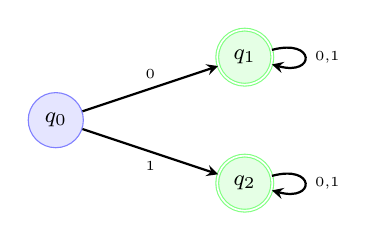
\begin{tikzpicture}[
  state/.style={circle, draw=blue!50, fill=blue!10, minimum size=0.7cm, font=\footnotesize},
  accept/.style={circle, draw=green!50, fill=green!10, minimum size=0.7cm, font=\footnotesize, double},
  arrow/.style={->, >=stealth, thick}
]
  \node[state] (q0) at (0,0) {$q_0$};
  \node[accept] (q1) at (2.4,0.8) {$q_1$};
  \node[accept] (q2) at (2.4,-0.8) {$q_2$};
  \draw[arrow] (q0) -- node[above, font=\tiny] {0} (q1);
  \draw[arrow] (q0) -- node[below, font=\tiny] {1} (q2);
  \draw[arrow] (q1) to[loop right] node[right, font=\tiny] {0,1} (q1);
  \draw[arrow] (q2) to[loop right] node[right, font=\tiny] {0,1} (q2);
\end{tikzpicture}
\caption{DFA non-minimal: $q_1$ dan $q_2$ ekuivalen}
\end{figure}

\subsection{Partisi dan Penggabungan}
\begin{table}[!htbp]
\centering
\begin{tabular}{|l|l|}
\hline
\textbf{Iterasi} & \textbf{Partisi} \\
\hline
$P_0$ & $\{q_1, q_2\}$ (final), $\{q_0\}$ (non-final) \\
\hline
$P_1$ & $\{q_1, q_2\}$, $\{q_0\}$ (tidak berubah) \\
\hline
\end{tabular}
\caption{Refinement partisi untuk contoh DFA}
\end{table}

Karena tidak ada pemisahan lebih lanjut, $q_1$ dan $q_2$ digabung menjadi satu state final.
